\casesection{One-dimensional planar free surface oscillations\label{case:thacker1d}}




\paragraph*{Purpose}
Flooding and drying are key phenomena from the hydraulic engineering practice. This test investigates the performance of \DFLOWFM for a case for which an exact solution is available.



\paragraph*{Linked claims}
Claims that are related to the current test case are:
\begin{itemize}
\item \clrefnoh{cl:generalGrids}
\item \clrefnoh{cl:advectionShortwave}
\item \clrefnoh{cl:advectionFloodingdrying}
\end{itemize}



\paragraph*{Approach}
For one-dimensional frictionless flow in a parabolic shaped basin, an exact solution is available for the evolution of the water level and the velocity, in case the initial surface elevation is a linearly increasing across the bathymetry. The analytical solution reads, with $x$ the coordinate across the bathymetry:
\begin{eqnarray*}
h(x,t)   &=& \frac{\eta h_0}{r_0} \left(2 x \cos \omega t - \eta r_0 \cos^2 \omega t  \right) \\
u(x,t)   &=& -\eta r_0 \omega \sin \omega t,
\end{eqnarray*}
with frequency $\omega = \sqrt{2gh_0}/r_0$ and period $2\pi/\omega$. This flow is simulated in \DFLOWFM and compared with the analytical solution. Basically, the only input parameters are $h_0$ as a vertical measure [m], $r_0$ as a horizontal measure [m] and $\eta$ a parameter [-]. The shape of the bathymetry is prescribed as:
\begin{equation*}
z(x) = -h_0 \left( 1-\frac{x^2}{r_0^2}  \right).
\end{equation*}



\paragraph*{Model description}
The model is set up as a one-dimensional case. Three grids are built: (1) a one-dimensional network (i.e.\ no cells, just linear pieces), (2) a one-dimensional grid (i.e.\ a row of cells) and (3) a two-dimensional grid, including squares of several sizes, connected by means of triangles. The three grids are shown in \autoref{fig:thacker1dgrid}.

\begin{figure}[h!]
\begin{center}

\includegraphics[width=1.0\columnwidth]{figures/grid.png}
\end{center}\caption{The three computational grids for the flooding and drying testcase.  \label{fig:thacker1dgrid}}
\end{figure}

The input settings $h_0$, $r_0$ and $\eta$ are 10 m, 120 m and 0.23 respectively. Friction and horizontal viscosity are turned off. The runtime comprises 600 seconds. Given the above parameters, the period $2\pi/\omega$ yields 53.8284 seconds. For the parameter \texttt{chkadvd}, the value of 0~m is set.




\paragraph*{Results}
The water level after 260 seconds (i.e.\ 4.83 periods) is shown in \autoref{fig:planar1dbasin} against the backdrop of the bathymetry as well as the analytical solution. The figure visualizes deviations between the computed solutions and the exact solution. The deviation is the most pronounced for the one-dimensional network. The one-dimensional grid and the two-dimensional grid show negligible differences mutually.

\begin{figure}[h!]
\begin{center}
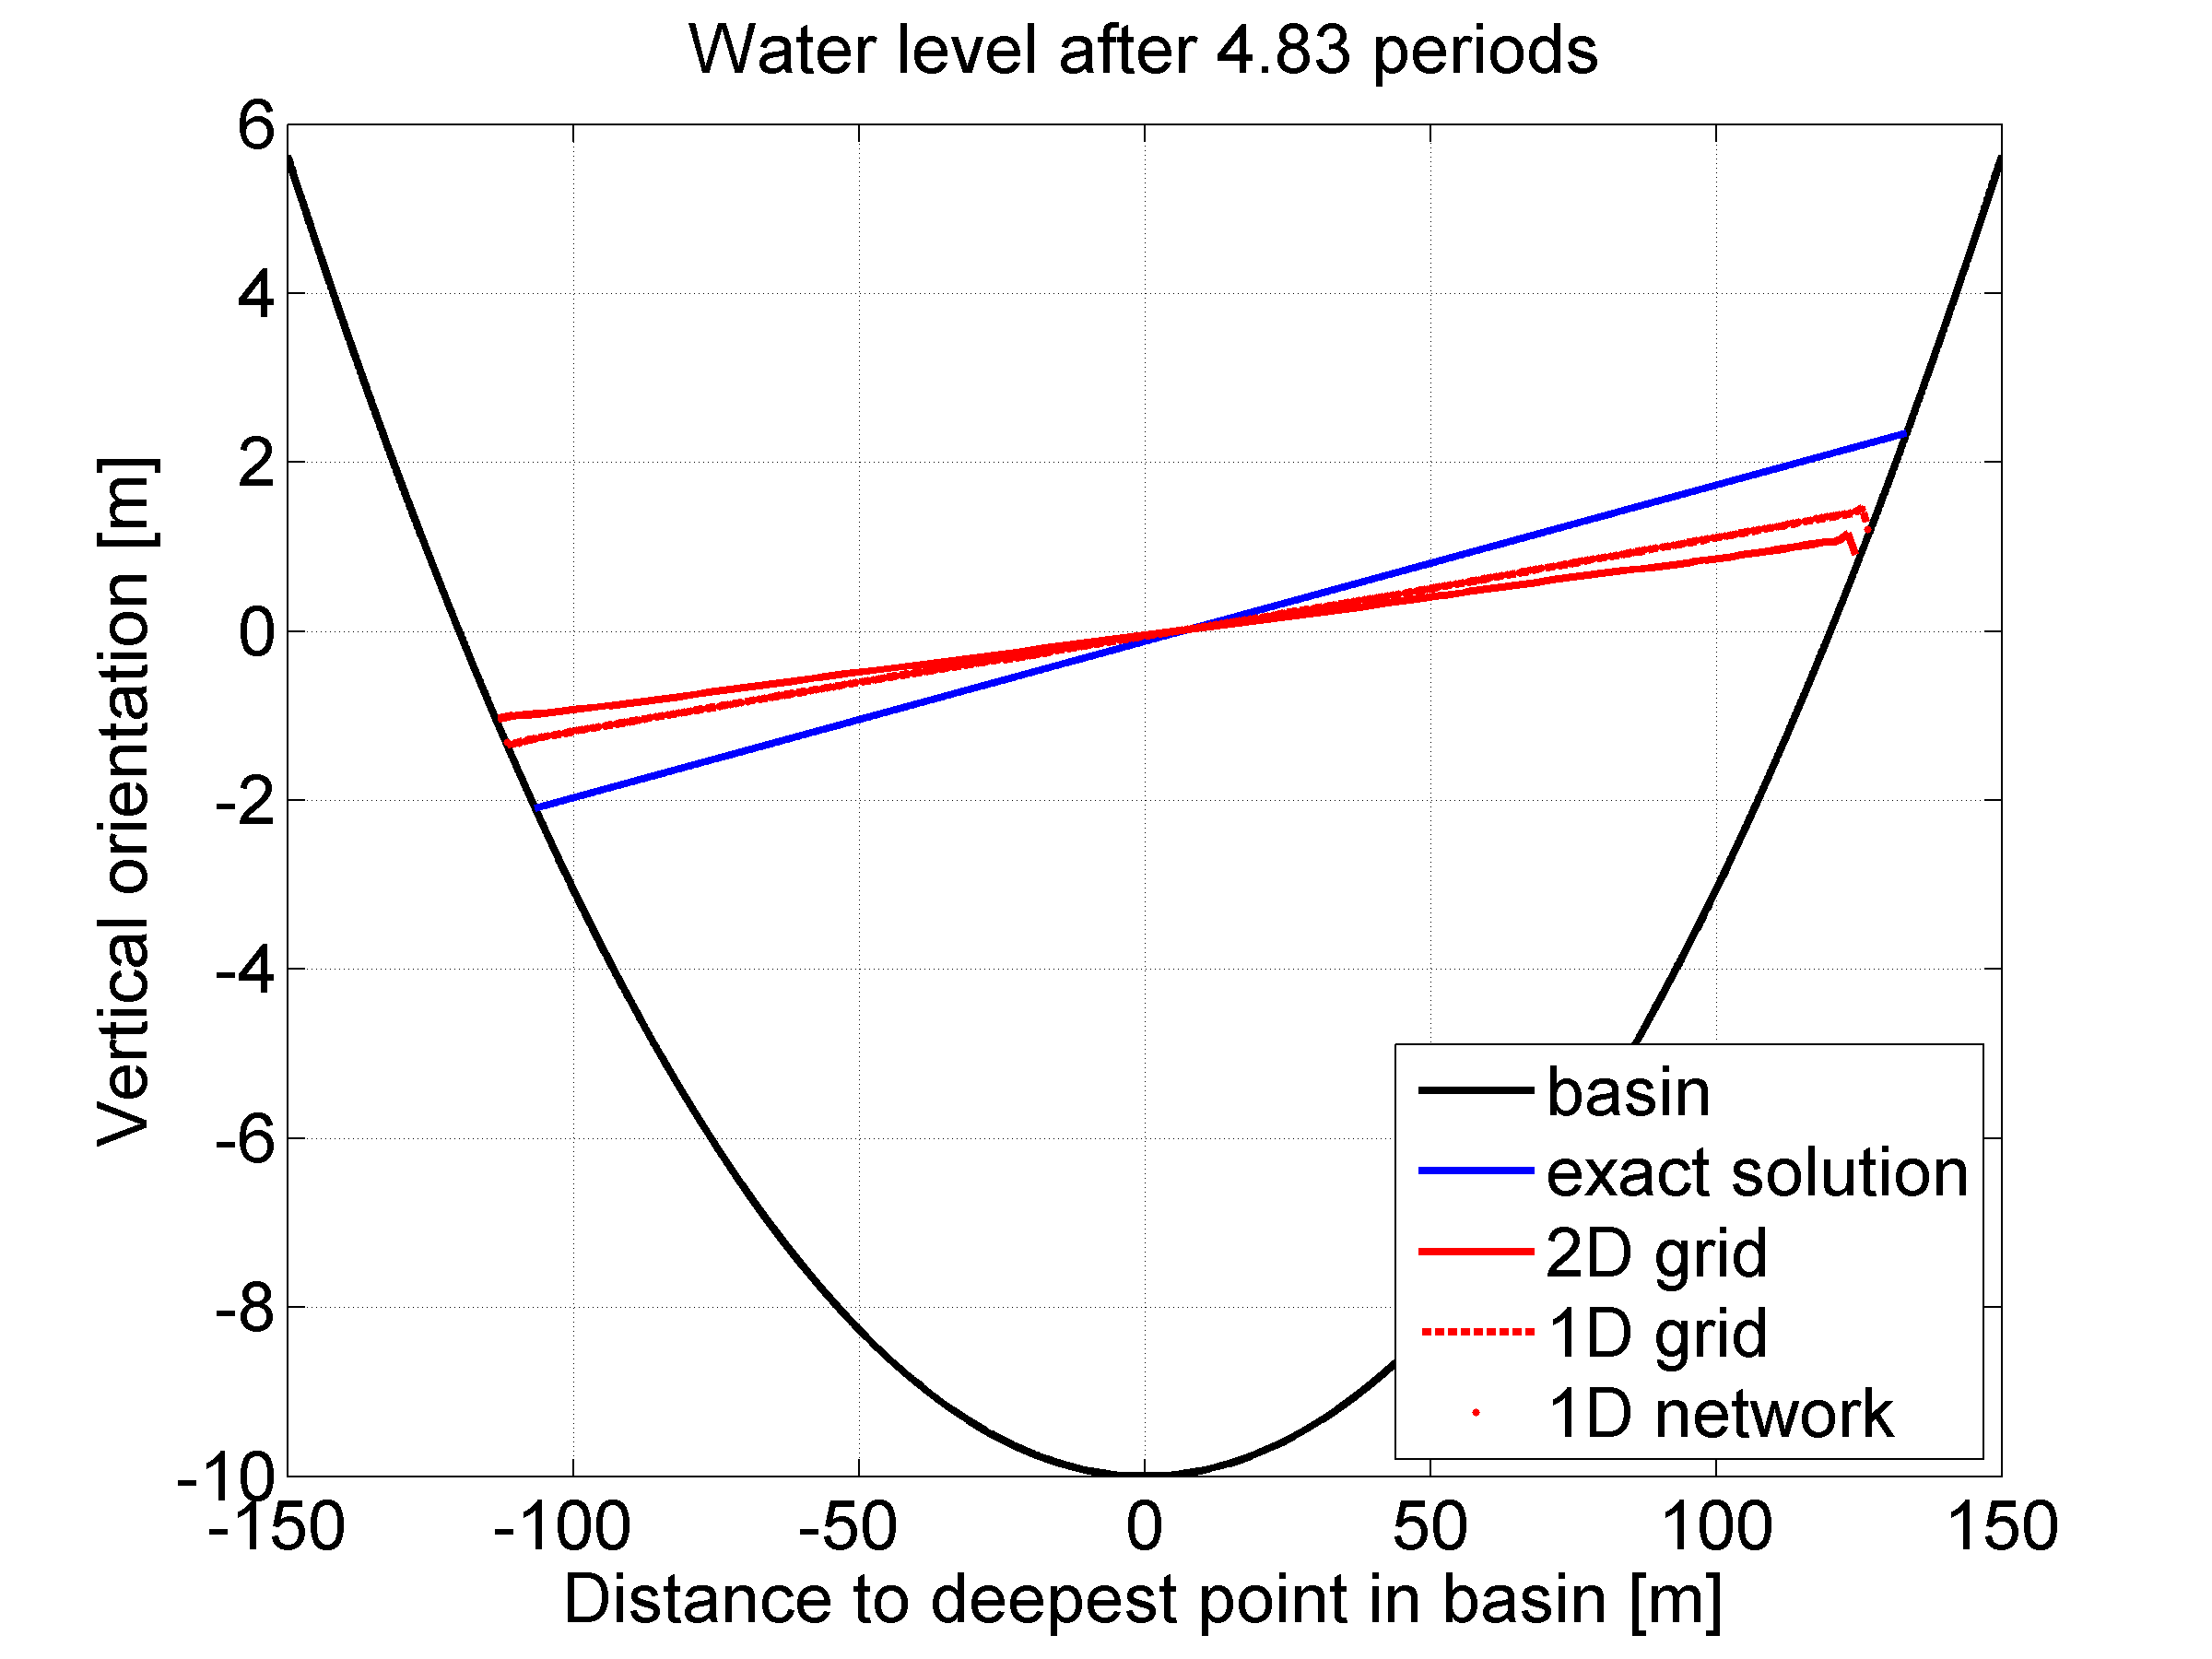
\includegraphics[width=0.57\columnwidth]{figures/planar1d.png}
\end{center}\caption{Computational results obtained on the one-dimensional network, the one-dimensional grid and the two-dimensional grid, drawn against the backdrop of the bathymetry. \label{fig:planar1dbasin}}
\end{figure}

\Autoref{fig:planar1dbasin} is provided a context through \autoref{fig:planar1dtime}. In \autoref{fig:planar1dtime}, the water level and the velocity are shown as varying in time. The location chosen for the comparison is 61.5 m right of the deepest point in the basin.
\begin{figure}[h!]
\begin{center}
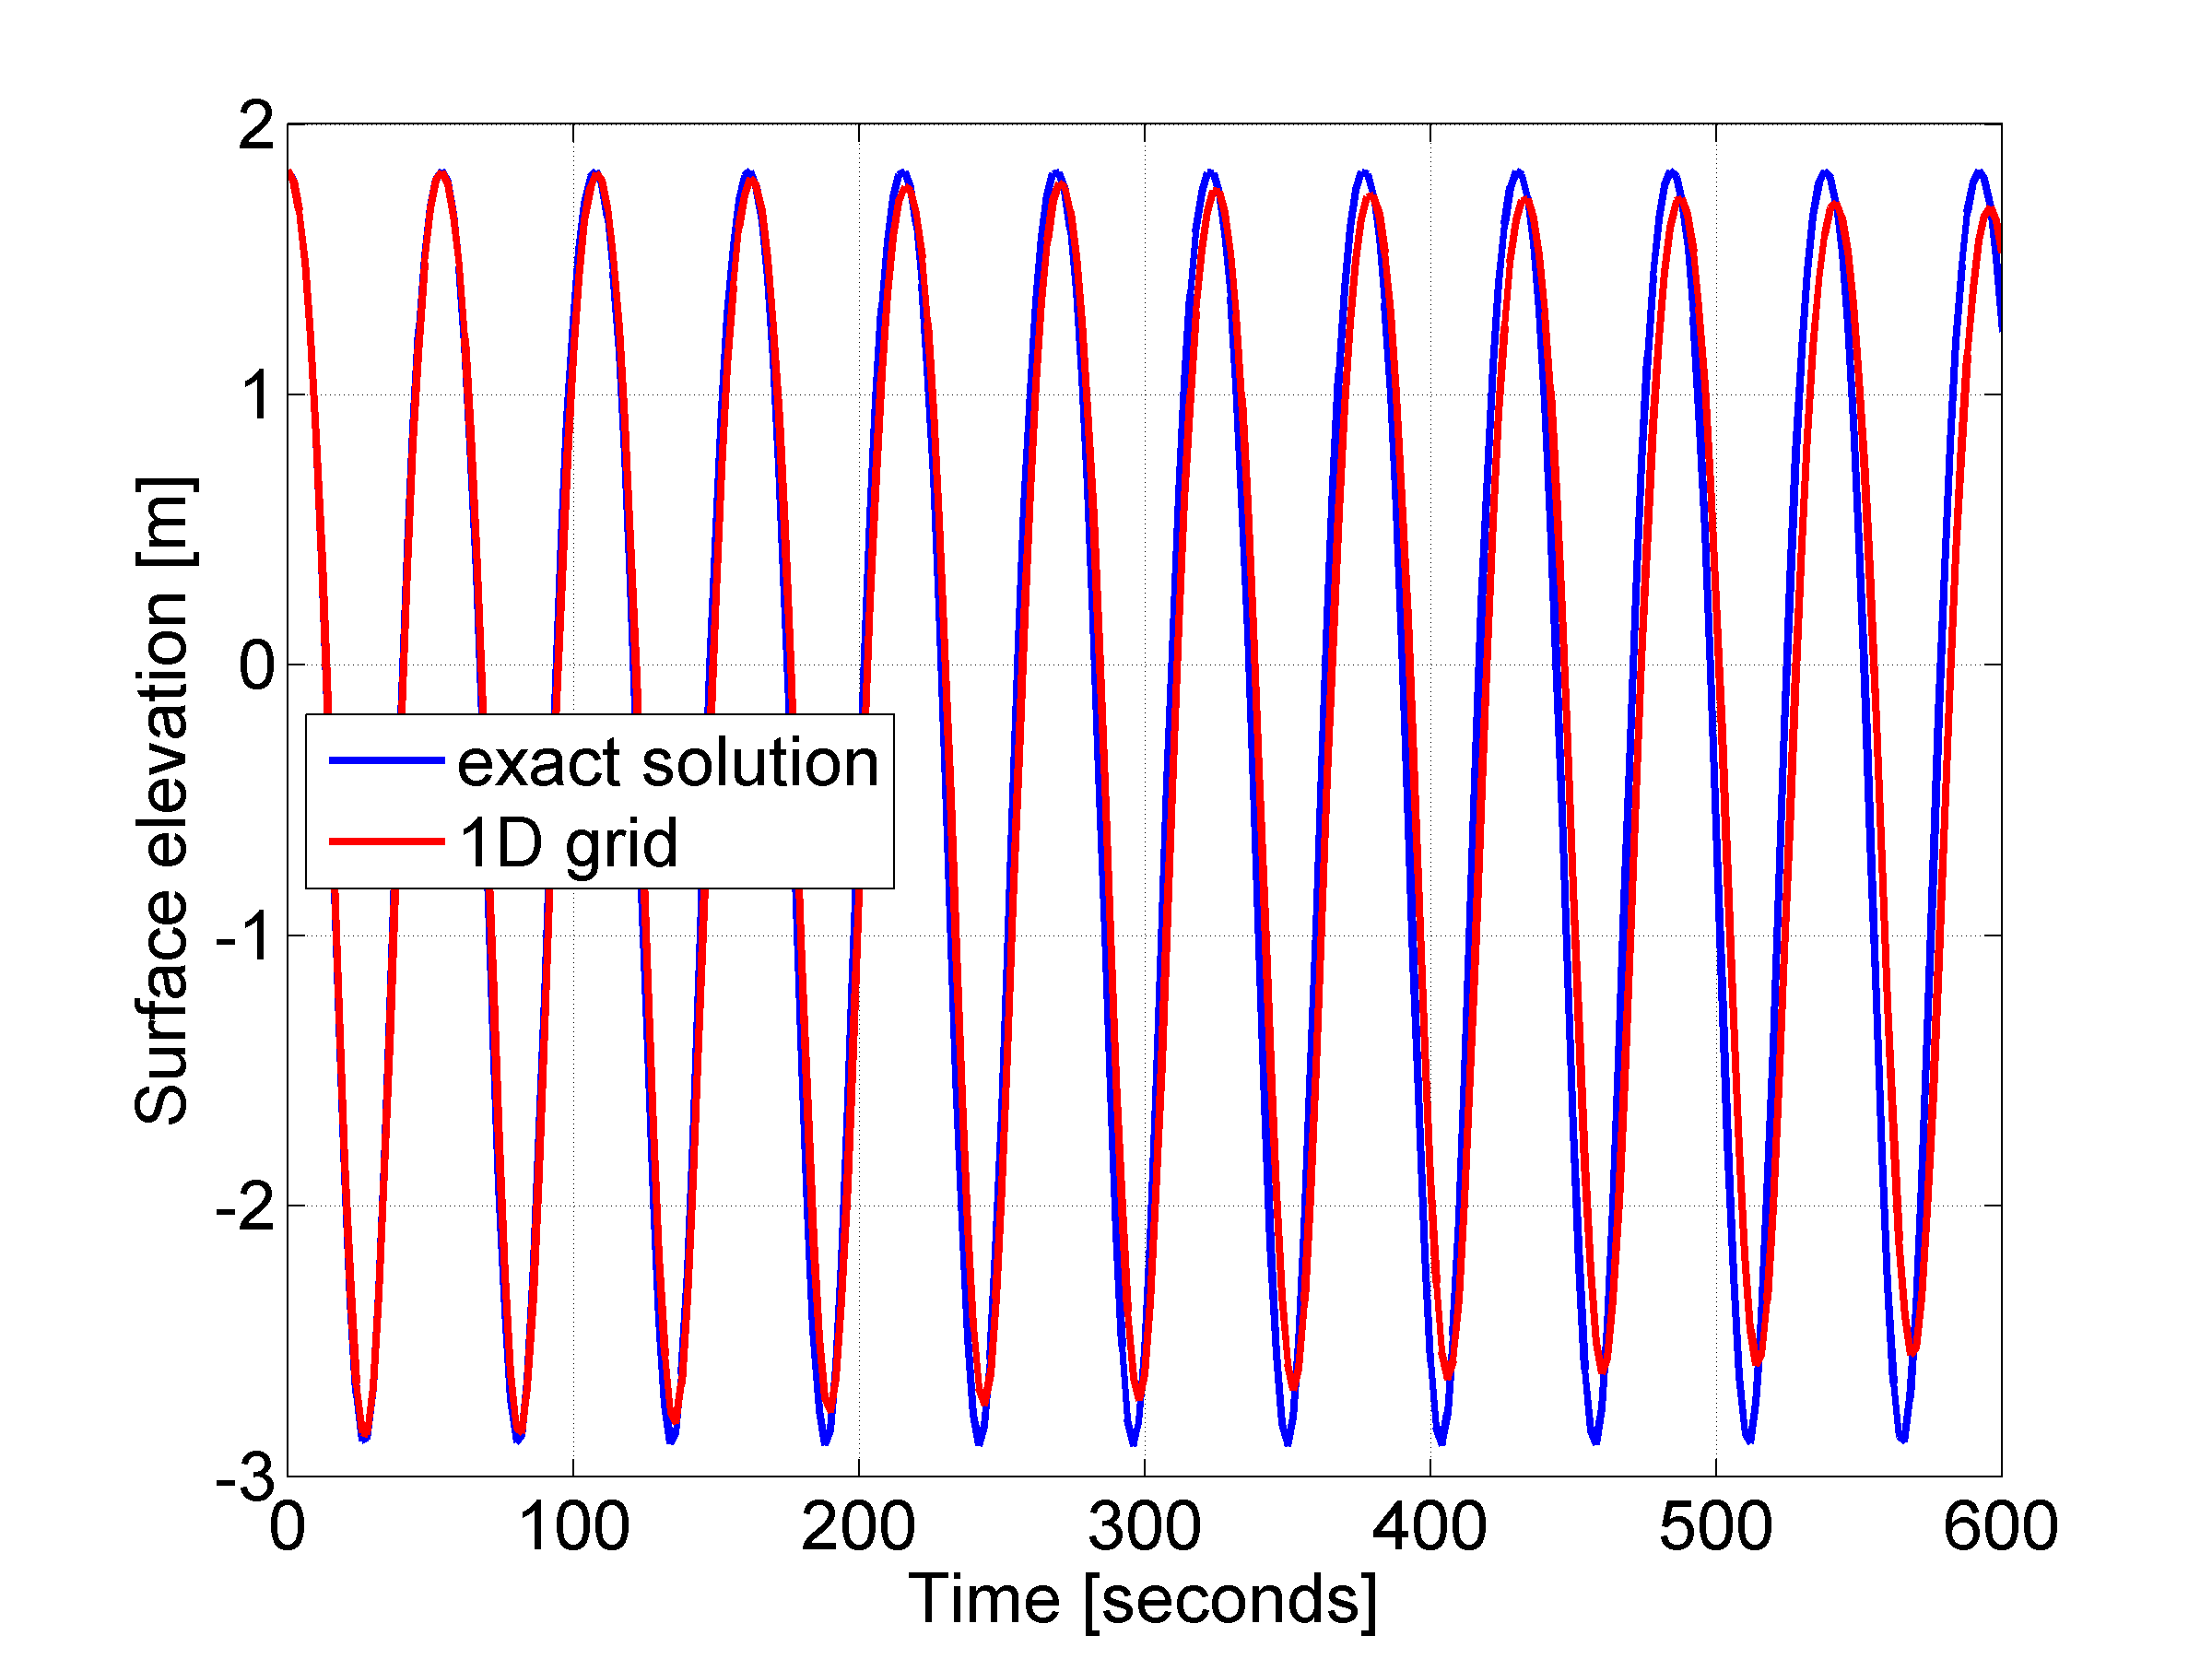
\includegraphics[width=0.49\columnwidth]{figures/planar1dwaterlevel.png}
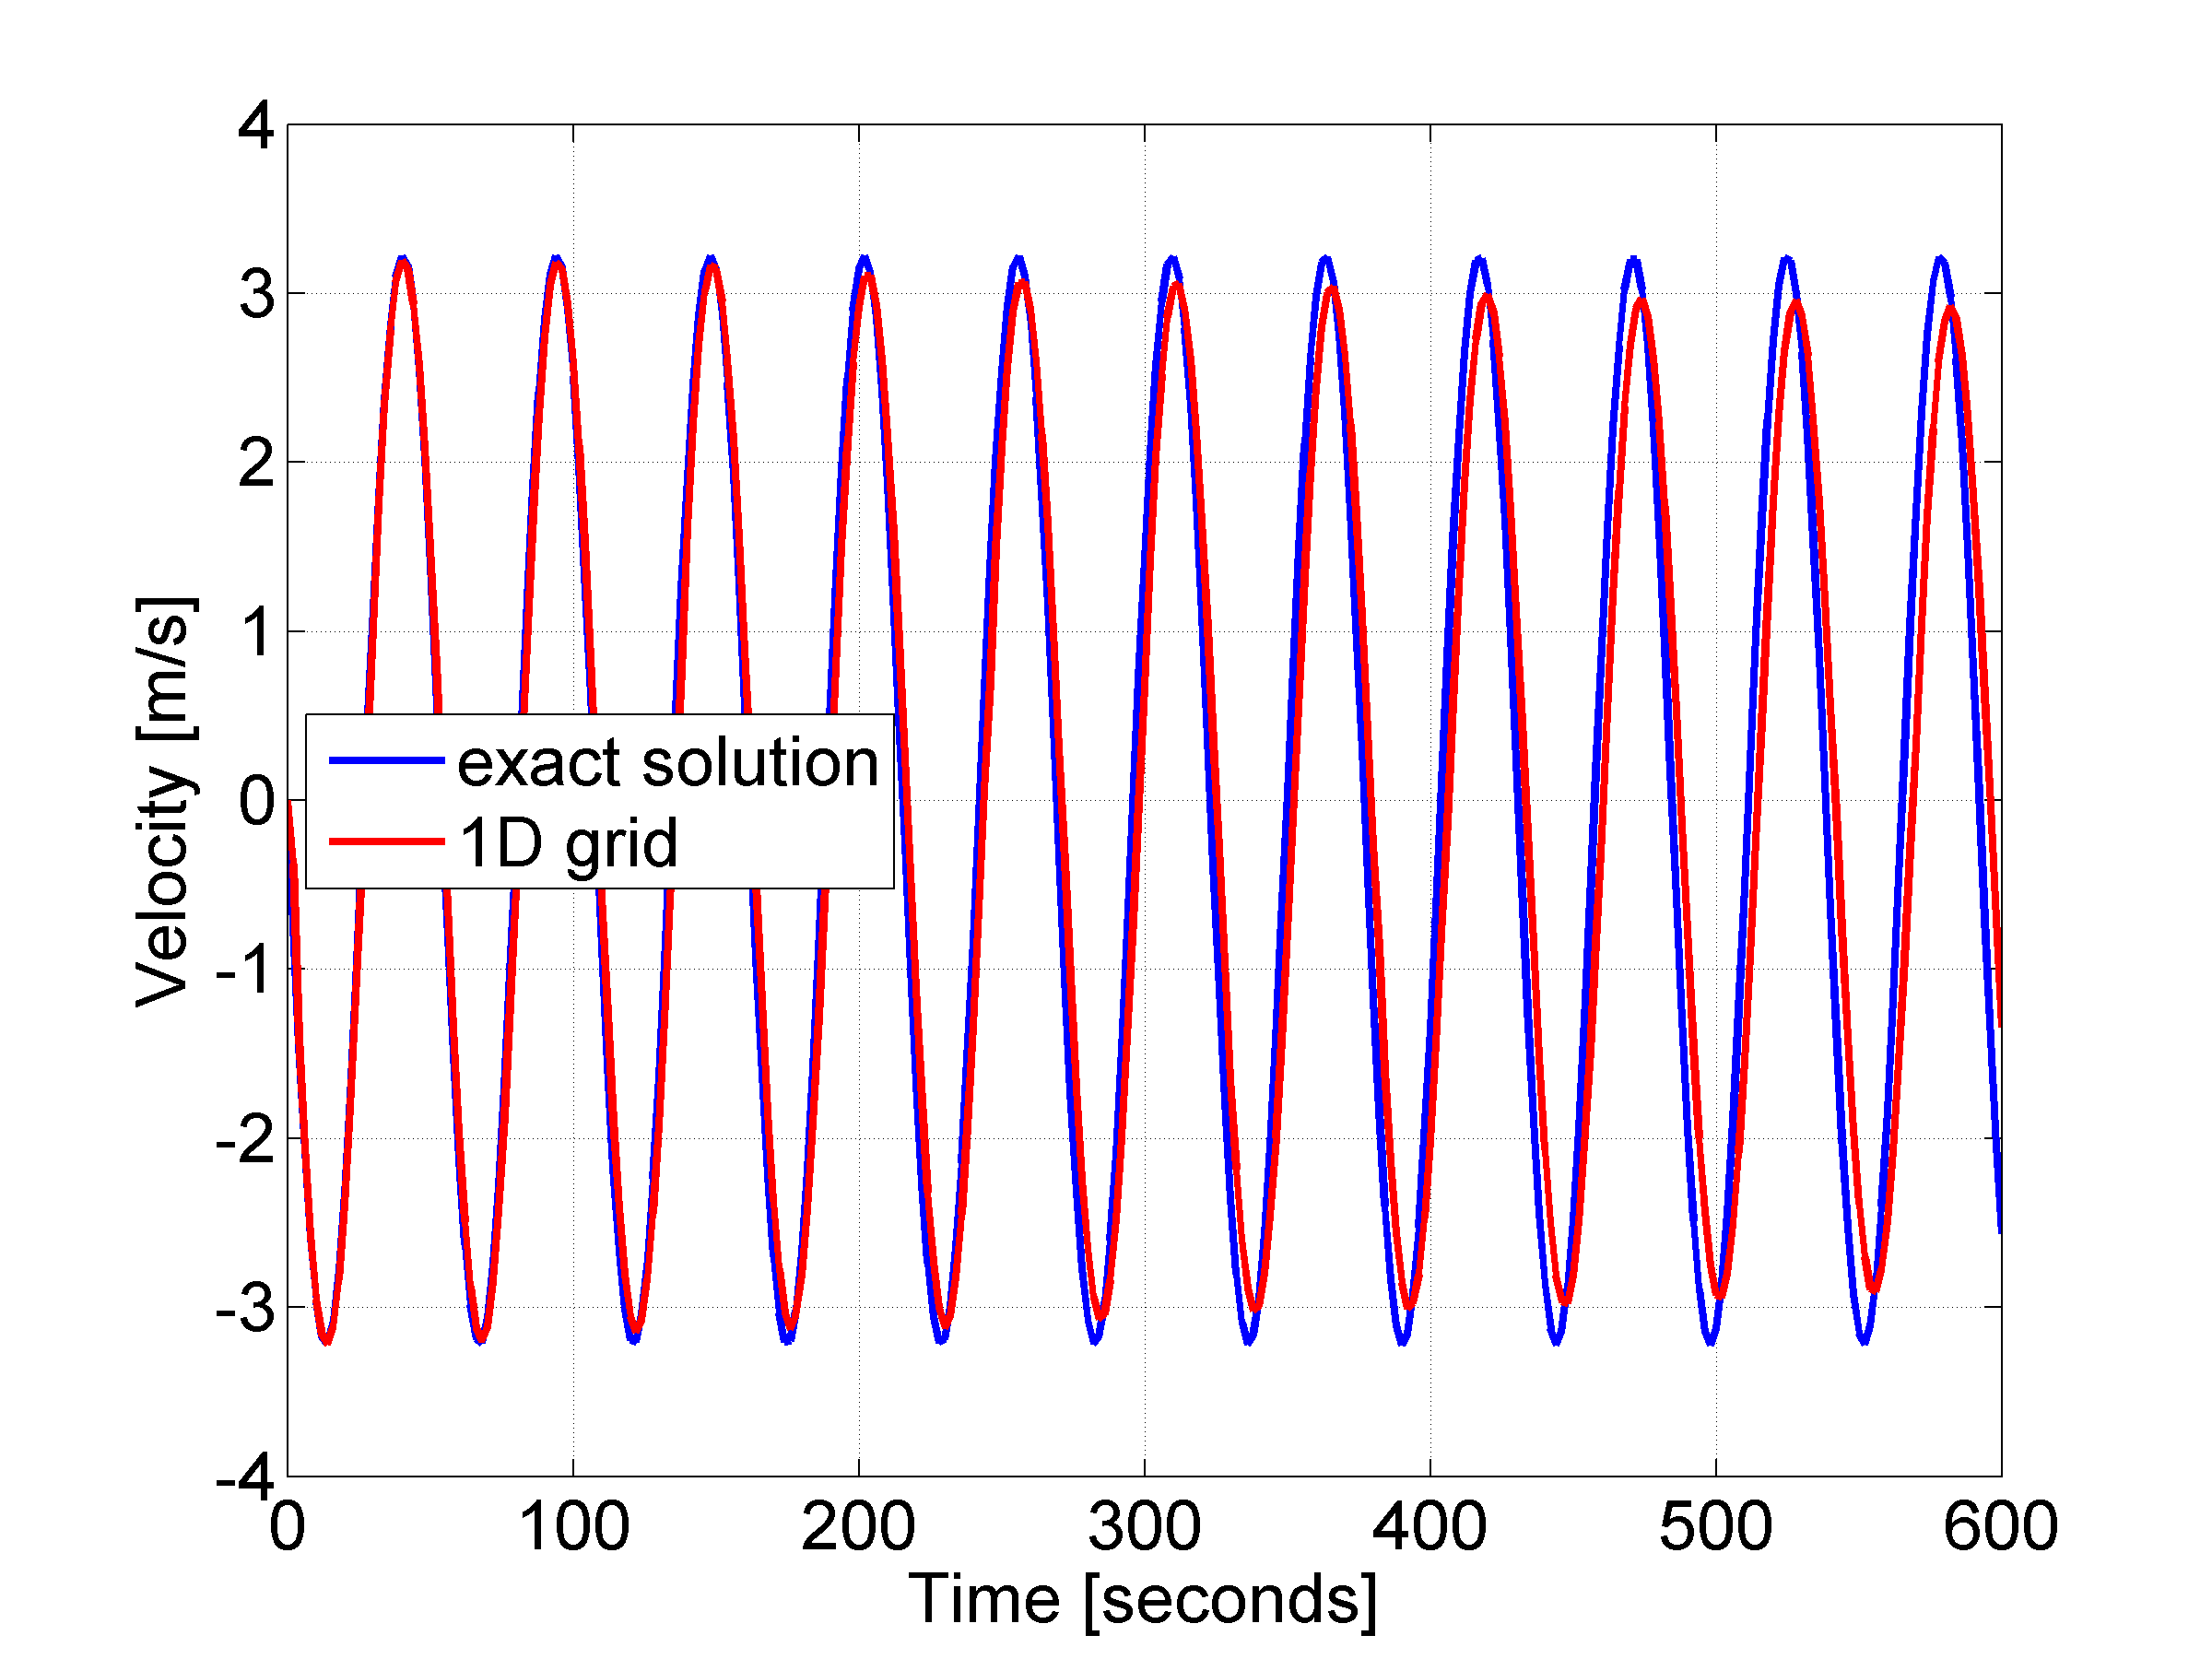
\includegraphics[width=0.49\columnwidth]{figures/planar1dvelocity.png}
\end{center}\caption{Temporal evolution of the water level (left panel) and the velocity (right panel) following from the computation on the one-dimensional grid and from the exact solution. \label{fig:planar1dtime}}
\end{figure}

\Autoref{fig:planar1dtime} shows that the amplitude of the computed signals decreases in time. Moreover, a phase lag appears with increasing magnitude in the course of time. Besides these general computational scheme related issues, the flooding and drying scheme appears to work properly in the sense that dry areas can flood and dry at all. 

As a variation on the same theme, grids are generated in addition with either square cells or triangular cells. In case of the use of triangular cells, it has been experienced that the choice on either \texttt{conveyance2D = 3} or \texttt{conveyance2D = -1} make quite a difference. In case of \texttt{conveyance2D = 3}, extreme velocities come into existence, whereas these stay absent in case of \texttt{conveyance2D = -1}. 

As an illustration, \autoref{fig:thacker1dconveyanceeffect} which displays the cell-center velocities in $x$-direction at 20 seconds after the start of the simulation. In these 20 seconds, some drying has taken place. The area over which this drying had taken place is marked by the arrow in \autoref{fig:thacker1dconveyanceeffect}. During these 20 seconds, high velocities have appeared on the interface dry/wet in case of \texttt{conveyance2D = -1}. However, extremely high velocities have appeared in the area that fell dry during these 20 seconds, in case of \texttt{conveyance2D = 3}. 

\begin{figure}[h!]
\begin{center}
\includegraphics[width=0.8\columnwidth]{../../c042_thacker1d_triangles/doc/figures/conveyanceeffect.png}
\end{center}\caption{Cell-center $x$-velocities at 20 seconds after the start of the simulation. For the top panel, \texttt{conveyance2D = -1} is used, for the bottom panel \texttt{conveyance2D = 3} is used. Notice the difference in color bar values (given in m/s). \label{fig:thacker1dconveyanceeffect}}
\end{figure}

The extremely high velocities have only appeared on triangular grids. Although the simulation have been carried out without friction, the extremely high velocities did not vanish after applying some amount of friction.



\paragraph*{Conclusion}
\dflowfm is able to computationally deal with flooding and drying, although a certain amount of diffusion takes place causing a phase lag with respect to the analytical solution. It is found that high velocities are found on the interface dry/wet. Moreover, it is found that the combination \texttt{conveyance2D = 3}, triangular grid and flooding/drying is a risky one.


\paragraph*{Version}
This test has been carried out with version dflow-fm-x64-1.1.148.41435.

